I battled a bit to set everything and in retrospect chapters like this should have been programmed as specials. However, as soon as they are set, adjustments are easily done.



%% Style 50

\cxset{style50/.style={
 name=,
 numbering=arabic,
 number font-size=\LARGE,
 number font-weight=\bfseries,
 number before={},
 number position=rightname,
 number dot=.,
 chapter color={black!80},
 chapter font-size=,
 chapter before=,
 number after=,
 chapter after=,
 number color=\color{black!80},
 title font-family=\rmfamily,
 title font-color=\color{black!80},
 title before=,
 title after=\par,
 title font-weight=\bfseries,
 title font-size=\LARGE,
 title beforeskip=\space,
 header style=empty,
 author block=true,
 author names=\textsc{James A. Russel and\\[-1.5pt] Jos\'e Miguel Fernandez-Dols },
 author block format=\normalfont\large,
 epigraph width=0.8\textwidth, epigraph align=left}}

\cxset{style50}
\chapter[Chapter Style Fifty]{Introduction to Chapter \\Style Fifty}

\epigraph{\raggedleft The human face -- in repose and in movement, at the moment of death as in life, in silence and in speech, when seen or seemed from within, in actuality or as recorded in art or recorded by the camera}{F. Ekman}

This is an unusual book with a rather unique style. The vertical rule is simple and breaks the monotony of a book that is heavy on text.
\begin{figure}[ht]
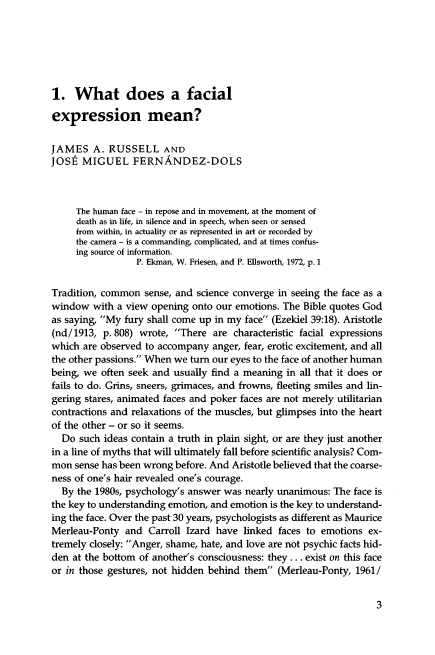
\includegraphics[width=0.48\textwidth]{./chapters/chapter50}\hfill
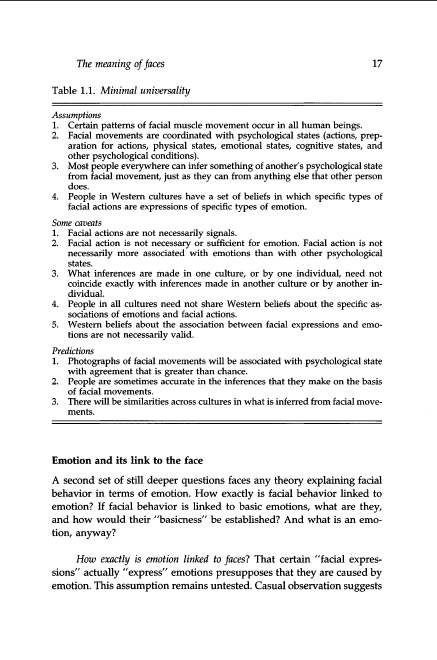
\includegraphics[width=0.48\textwidth]{./chapters/chapter50a}
\caption{Style 50 from the Oxford Handbook of Cuneiform Culture.}
\end{figure}

This style is very modern and typical of many computer books. The difficulty is in integrating all the page elements to make it work flawlessly.

The psychology of facial
expression
Edited by
James A. Russell
University of British Columbia
Jose Miguel Fernandez-Dols
Universidad Autonoma de Madrid, Cambridge University Press.

